\documentclass[aspectratio=169,11pt]{beamer}
\usetheme{Madrid}
\usecolortheme{seahorse}
\setbeamertemplate{navigation symbols}{}
\setbeamertemplate{footline}[frame number]
\usepackage{booktabs}
\usepackage{amsmath}
\usepackage{graphicx}
\usepackage{xcolor}
\definecolor{good}{HTML}{1baf7a}
\definecolor{bad}{HTML}{e34948}
\definecolor{hub}{HTML}{2a78d6}

\title{Architectures of problem solving}
\subtitle{\small (working notes for discussion)}
\author{}
\date{July 2026}

\begin{document}

\begin{frame}
  \titlepage
\end{frame}

% ------------------------------------------------------------------
\begin{frame}{Where we started}
 
  \begin{itemize}
    \item Agents on a fixed directed network share a drifting Boolean-satisfiability task:
          private assignments $x^{(i)} \in \{0,1\}^K$, a hidden clause set $\mathcal{C}$
          ($M=\alpha K$; one clause replaced every $\tau$ ticks).
    \item Two learning channels: \textbf{private observation} (rate $p_{\text{obs}}$) and
          \textbf{communication} (receiver-pull from in-neighbours), with the per-agent rate
          normalised across topologies: $s = 1/\langle k_{\text{in}}\rangle$.
   \item Upon learning about a new clause, each agent would try flipping the variables in their private assigments that are involved and keep the change if it reduces the number of known clauses violated (local greedy optimisation)
    %\item Headline result: with communication volume controlled, \alert{long-run performance
          %is topology-independent} --- random, small-world, scale-free, hierarchical all
         % converge to the same violation level.
  \end{itemize}
  \vspace{4pt}
  %\begin{block}{The nagging question}
  %  Is that a deep property of distributed problem solving --- or an artefact of what
  %  communication was actually carrying?
  %\end{block}
\end{frame}

% ------------------------------------------------------------------
\begin{frame}{Examining the behaviour of information inside the model...}
   \textbf{Observation: after a number of ticks, the network was filled with mostly stale information.}
  %\begin{columns}[T]
   % \begin{column}{0.52\textwidth}
      \begin{itemize}\small
        \item Nothing ever removes a clause from a knowledge base: once learned,
              a clause \emph{outlives its own death} in $\mathcal{C}$ and keeps being
              re-transmitted as if new.
        \item $\sim$70\% of held knowledge was stale (i.e. false) by $t=2000$ at $\tau=10$;
              %\alert{80--85\% under fast drift ($\tau=1$)}.
        \item Communication --- the only structure-\emph{dependent} channel --- was
              mostly noise; the only reliable truth source was private observation,
              which is structure-\emph{independent}.
      \end{itemize}
      \small $\Rightarrow$ With 4 in 5 communicated clauses dead on arrival, no topology could
      have differentiated itself.
        \vspace{4pt}
      \\
      \textbf{While we couldn't know for sure that this was uniquely driving the result, we do know that - with communicated information comprising of fake news - the model couldn't behave otherwise}
%    \end{column}
 %   \begin{column}{0.48\textwidth}
  %    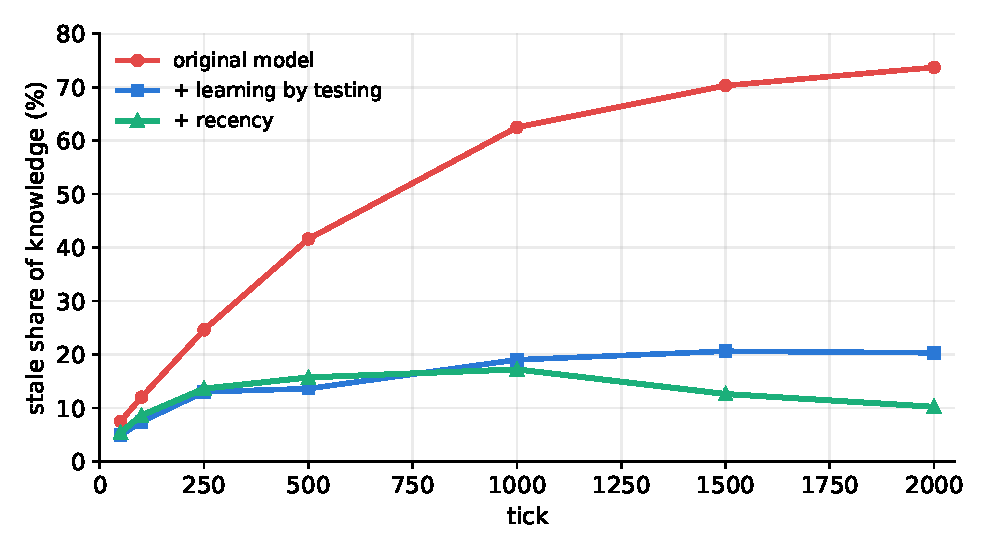
\includegraphics[width=\linewidth]{figs/stale_trajectory.pdf}
   %   \par\centering\scriptsize Stale share of knowledge bases (Scale Free, $\tau=10$, 5-seed means).
   % \end{column}
  %$\end{columns}
\end{frame}

% ------------------------------------------------------------------
\begin{frame}{Tweak 1 --- "learning by testing" (signed beliefs)}
  Replaces passive observation with \textbf{active verification}. Each tick, with equal
  probability, the agent either:
  \begin{enumerate}
    \item \textbf{tests a new clause}: draws a candidate from the universe of possible
          clauses ($K(K-1)$ of them) that it holds no belief about, and keeps it as a
          \emph{positive belief} iff it actually exists in $\mathcal{C}$; or
    \item \textbf{tests a belief held in its knowledge base} (positive or negative): if they find that a clause does not exist any longer, the clause is kept as a \emph{negative belief} (i.e., ``this constraint no longer exists'').
  \end{enumerate}
  \vspace{2pt}
  \begin{itemize}
    \item $\Rightarrow$ Knowledge base holds \textbf{signed beliefs}: beliefs about a clause existing, and beliefs about a clause not existing. 
      \begin{itemize}
        \item Only positive beliefs drive the greedy optimisation.
        \item Size of the knowledge set was doubled to $2M$ (this is relatively arbitrary)
      \end{itemize}
    \item Communication transmits \textbf{both polarities}: the receiver adopts the
          sender's sign on a clause they disagree about.
    
  \end{itemize}
   The idea is to let the network flush fake news.
\end{frame}

% ------------------------------------------------------------------
\begin{frame}{Tweak 2 --- ``communication recency'' (transmit the most recently learned belief) }
  \begin{block}{Recency rule}
    Upon communication, the sender passes on its most recent belief --- most
    recently learned --- among those the receiver doesn't share. Freshest news travels first; old items
    are forwarded only once everything newer is already shared.
  \end{block}
  \vspace{2pt}
 
  \vspace{4pt}

  \textbf{Effect on information quality} (share of held positives that are stale):
  \begin{center}\small
  \begin{tabular}{@{}lcc@{}}
  \toprule
   & original model & learning by testing \& recency \\
  \midrule
  slow drift ($\tau=10$) & $\sim$70\% & \textcolor{good}{$\sim$10\%} \\
  fast drift ($\tau=1$) & $\sim$80\% & \textcolor{good}{$\sim$40--50\%} \\
  \bottomrule
  \end{tabular}
  \end{center}
  {\small Stale information now disappears within a few hundred ticks of a clause's
  death: communication carries mostly \emph{live} content. \\
  Most importantly, network structure likely to play a role, as better connected individuals get good information more quickly}
\end{frame}

% ------------------------------------------------------------------
\begin{frame}{The tweaks in action: stale information is flushed}
  \centering
  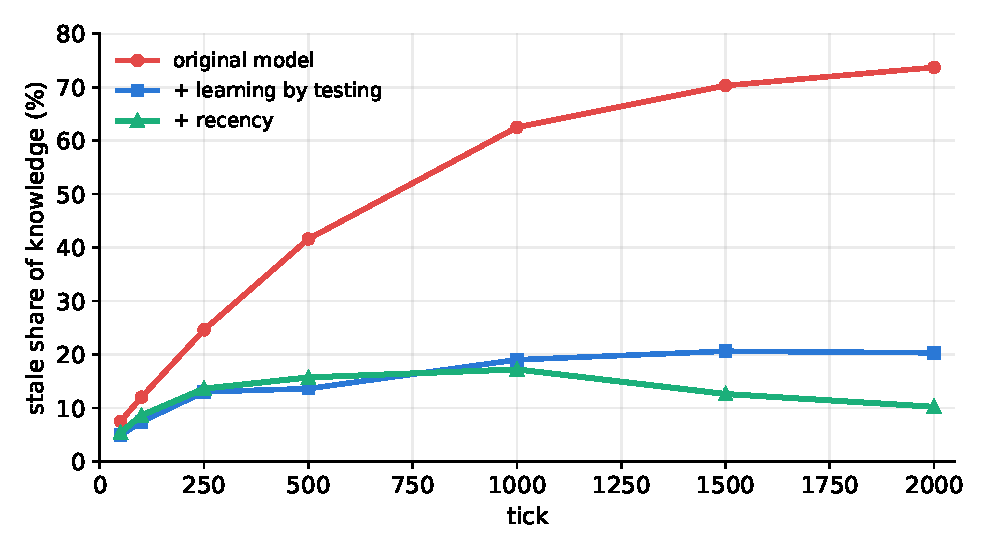
\includegraphics[width=0.6\linewidth]{figs/stale_trajectory.pdf}

  \vspace{4pt}
  {\small In the original model stale knowledge climbs without bound ($\sim$74\% by
  $t=2000$). Learning by testing flushes most of it ($\sim$20\%); transmitting the
  freshest belief first (recency) roughly halves what remains ($\sim$10\%).}

  \vspace{2pt}
  {\scriptsize Scale Free, $\tau=10$, 5-seed means. Each tweak is added on top of the previous.}
\end{frame}

\begin{frame}{New default configuration}


 \textbf{Default configuration} from here on: $N=80$, $K=30$, $\alpha=2$,
  \alert{$\tau=1$ (fast drift)}, $T=2000$, communication normalised, testing + recency on;
  10 seeds; long run $=$ last 500 ticks.

  \vspace{6pt}
  Fast drift increases the churn of information, making structure more important (I hope).
\end{frame}  

% ------------------------------------------------------------------
\begin{frame}{Two hypotheses}
  \begin{block}{H1 --- Structure}
    Does the \emph{shape} of the network --- random, small-world, scale-free,
    hierarchical --- change collective performance?
  \end{block}
  \vspace{8pt}
  \begin{block}{H2 --- Position}
    Does an agent's \emph{location} in the network --- central vs.\ peripheral ---
    change its relative performance?
  \end{block}
  \vspace{8pt}
  \centering\small Both are ``yes'' in organisation theory. We test them
  with communication volume held equal across networks.
\end{frame}

% ------------------------------------------------------------------
\begin{frame}{H1 (structure): \textcolor{bad}{denied}}
  \begin{columns}[T]
    \begin{column}{0.46\textwidth}
      Four topologies, matched intake ($\langle k_{\text{in}}\rangle \approx 4$),
      10 seeds. Long-run performance is the same everywhere:
      \begin{itemize}\small
        \item average violations 28.9--29.6
        \item best-agent violations 20.2--20.4
        \item homogeneity 0.69--0.72
      \end{itemize}
      \vspace{6pt}
      Gaps are within seed noise -- at least under the normalisation of communication rate. \\
      
      The fixes to the model didn't change this, so independence is not
      an artefact of stale information. It seems to be a featrue of the model. \\
      It's supported by the theory derivations.
    \end{column}
    \begin{column}{0.54\textwidth}
      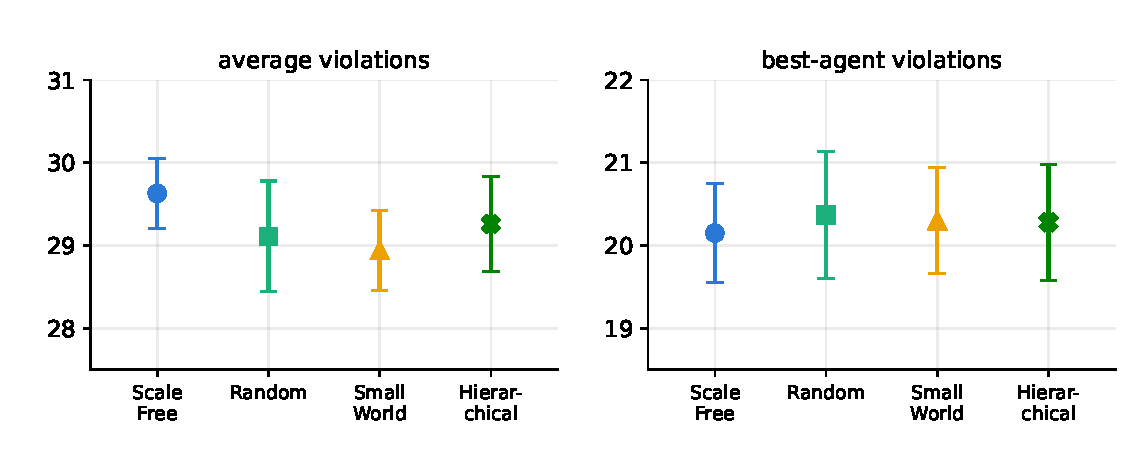
\includegraphics[width=\linewidth]{figs/h1_topology.pdf}
    \end{column}
  \end{columns}
\end{frame}

% ------------------------------------------------------------------
\begin{frame}{H2 (position): \textcolor{good}{validated}}
  \begin{columns}[T]
    \begin{column}{0.46\textwidth}
      \emph{Population} average performances might be equalised, but each agent's performance 
      scales with its own in-degree.
      \vspace{6pt}
      \begin{itemize}\small
        \item central agents have fewer violations in \textbf{40/40 runs}
              ($\rho \approx -0.5$ to $-0.6$).
      \end{itemize}
      \vspace{6pt}
      \textbf{Performance vs.\ in-degree is one curve, shared by every topology.}
      Structure only decides which points on it exist.
    \end{column}
    \begin{column}{0.54\textwidth}
      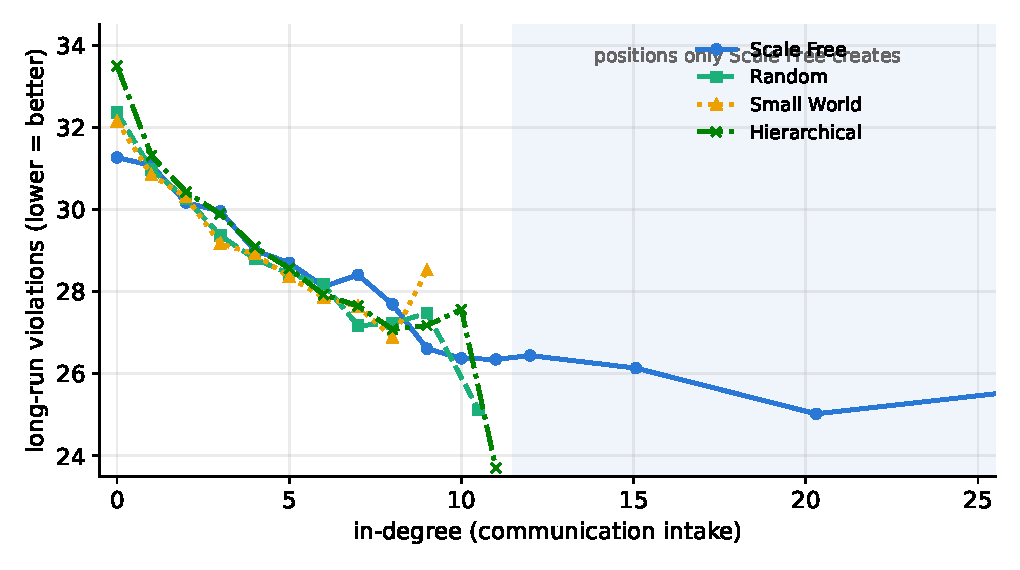
\includegraphics[width=0.97\linewidth]{figs/curve_lbt.pdf}
    \end{column}
  \end{columns}
\end{frame}

% ------------------------------------------------------------------
\begin{frame}{Why the original model hid this}
  \centering
  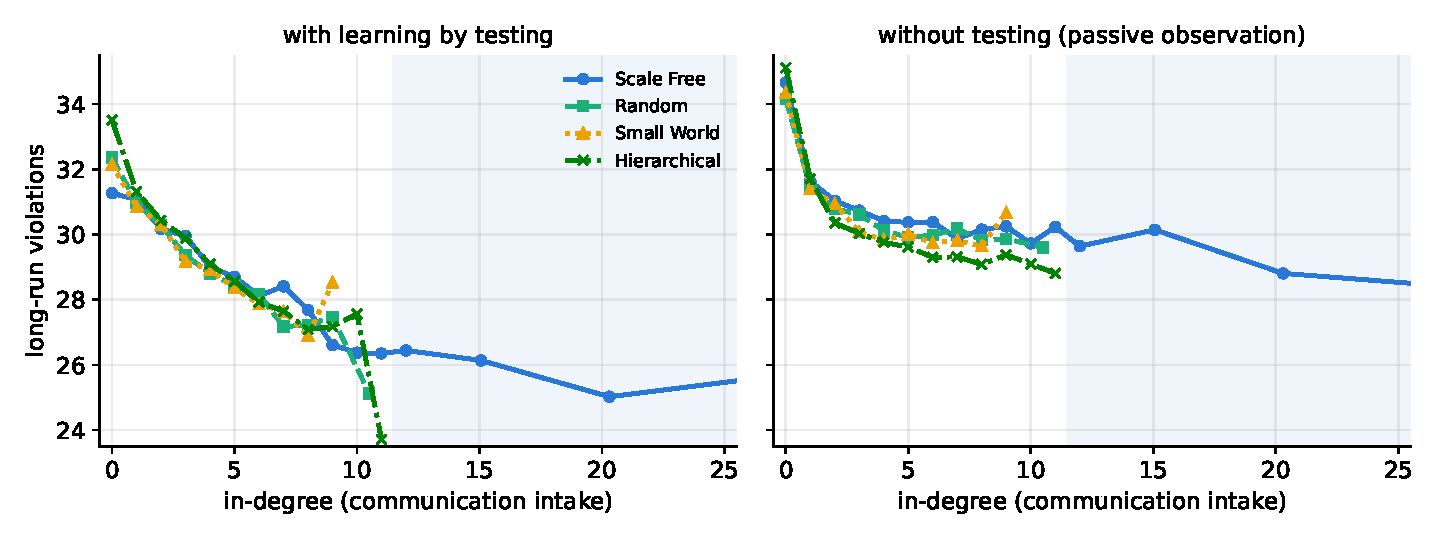
\includegraphics[width=0.72\linewidth]{figs/curve_compare.pdf}
  \vspace{4pt}

  {\small With testing (left), communication yields \emph{useful} data and the curve keeps
  falling. Without it (right), most communication is fake news --- past the first
  links, more intake adds nothing. In other words, position pays only once information is trustworthy.}
\end{frame}

% ------------------------------------------------------------------

\begin{frame}{Position pays across the whole range (designed uniform-degree net)}
 \center
  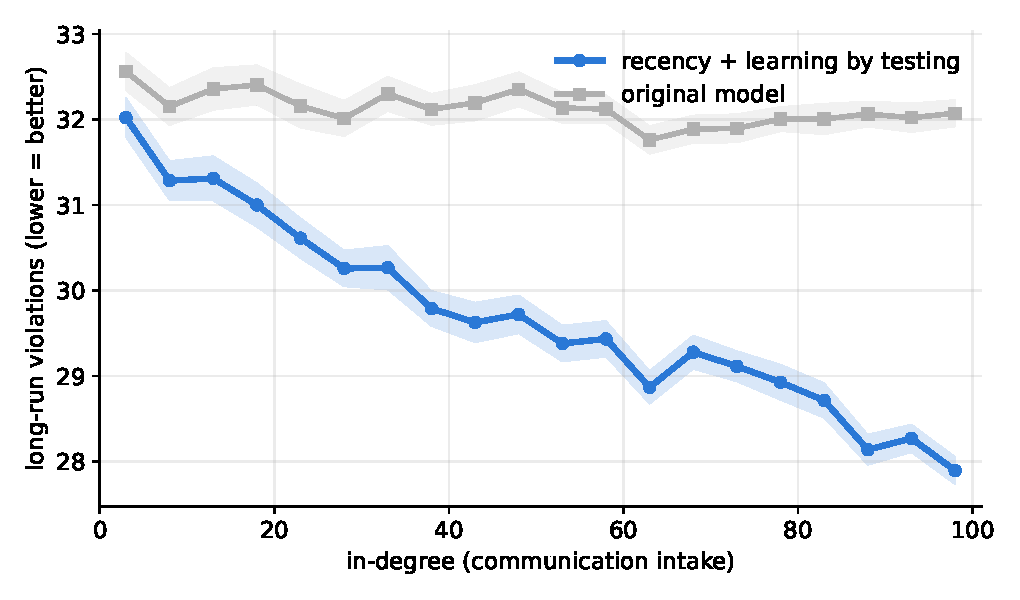
\includegraphics[width=0.65\linewidth]{figs/curve_uniform_degree.pdf}
  \par I believe the milder slope reflects this network's high average degree: under normalisation ($s=1/\langle k_{\text{in}}\rangle$) a given in-degree carries less data. So it's the same curve stretched over a wider axis.
\end{frame}

% ------------------------------------------------------------------
% (Recap slide removed --- the two hypotheses are now stated up front,
%  and each verdict lives on its own H1 / H2 result slide.)

% ------------------------------------------------------------------
\begin{frame}{Implication for organisation design}
  \begin{itemize}
    \item Centralisation does not raise average performance: strong hubs are
          paid for by a larger weak periphery.
    \item However, network structure can buy \textbf{intentionality}. If decision-making or control rights are scarce, one can design organisations centralised around decision makers. Other things being equal, this guarantees better performances (i.e., more accurate problem solving).
  \end{itemize}
  \vspace{10pt}
 % \begin{block}{}
 %   \centering When decision rights or control are scarce, centralised structures let you
  %  \emph{place} them on the agents who will perform best. Flat structures leave it to chance.
  %\end{block}
\end{frame}

% ------------------------------------------------------------------
\begin{frame}{But the theory currently says position shouldn't matter}
  {\small The degree-resolved mean field (Atiyab):}
  \[ \frac{dp_k}{dt} = R_k\bigl[(1-p_k)\Pr(Z>0) - p_k\Pr(Z<0)\bigr] \]
  {\small At steady state the bracket vanishes, so the rate $R_k$ cancels: every degree
  class reaches the same $p_k^{\star}$. Position should set only the \emph{speed} of
  convergence --- yet the simulation shows a lasting position gradient.}
  \vspace{8pt}
  \begin{block}{Where the gap likely hides}
    The ODEs let every agent sample the same clause distributions and treat all held
    clauses as true. But the true binding quantity is \emph{validity}, which rises
    with intake and is therefore $k$-dependent. A validity state $q_k$ (plus the
    negative-belief channel) might recover the gradient.
  \end{block}
\end{frame}

\end{document}
